\setlength{\fboxrule}{2pt}
\newcommand\fboxg{\fcolorbox{green}{white}}
\newcommand\fboxr{\fcolorbox{red}{white}}

\begin{figure}[t]
	\centering
	\addtolength{\tabcolsep}{-4.5pt}
	\begin{tabular}{cccc}
		Photo & \textit{Leather} Prior & \textit{Plaster} Prior & \textit{Wood} Prior
		\\
		\begin{overpic}[width=0.85\resultwidth]{real/leather_3/target.jpg}
			\imglabel{Leather-5}
		\end{overpic} &
		\fboxg{\includegraphics[width=0.85\resultwidth]{real/leather_3/good1.jpg}} &
		\fboxr{
\includegraphics[width=0.85\resultwidth]{mismatch/2_leather5/plaster.png}} &
		\fboxr{
\includegraphics[width=0.85\resultwidth]{mismatch/2_leather5/wood.png}} 
		\\[5pt]
		\begin{overpic}[width=0.85\resultwidth]{real/wood_3/target.jpg}
			\imglabel{Wood-5}
		\end{overpic} &
		\fboxr{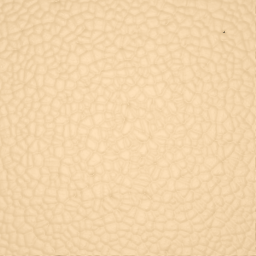
\includegraphics[width=0.85\resultwidth]{mismatch/6_wood5/leather.png}} &
		\fboxr{
\includegraphics[width=0.85\resultwidth]{mismatch/6_wood5/plaster.png}} &
		\fboxg{\includegraphics[width=0.85\resultwidth]{real/wood_3/good1.jpg}} 
	\end{tabular}
	\captionsetup{labelfont=bf,textfont=it}
	\caption{\label{fig:Mismatch}
		\revision{
			\textbf{Comparison} with mismatched forward models. With an inappropriate model as the prior, it would only match the global color but missing all the details.   
		}
	}
\end{figure}